\section{position}\label{position}

ToDo:
\begin{enumerate}[nosep]
    \item Erklärung Features
    \item Performance Hillas
    \item ML Trainingsperformance + daten
    \item Ergebnisse Mono
    \item Ergebnisse Stereo, Probleme
    \item Vergleich Hillas/Disp
\end{enumerate}

% jeweils features und r2,  ggf accuracy
% test: r2, sensitivity vs energy und vs multi bei stereo
\subsection{Analysis for the mono-lst}
\begin{figure}
    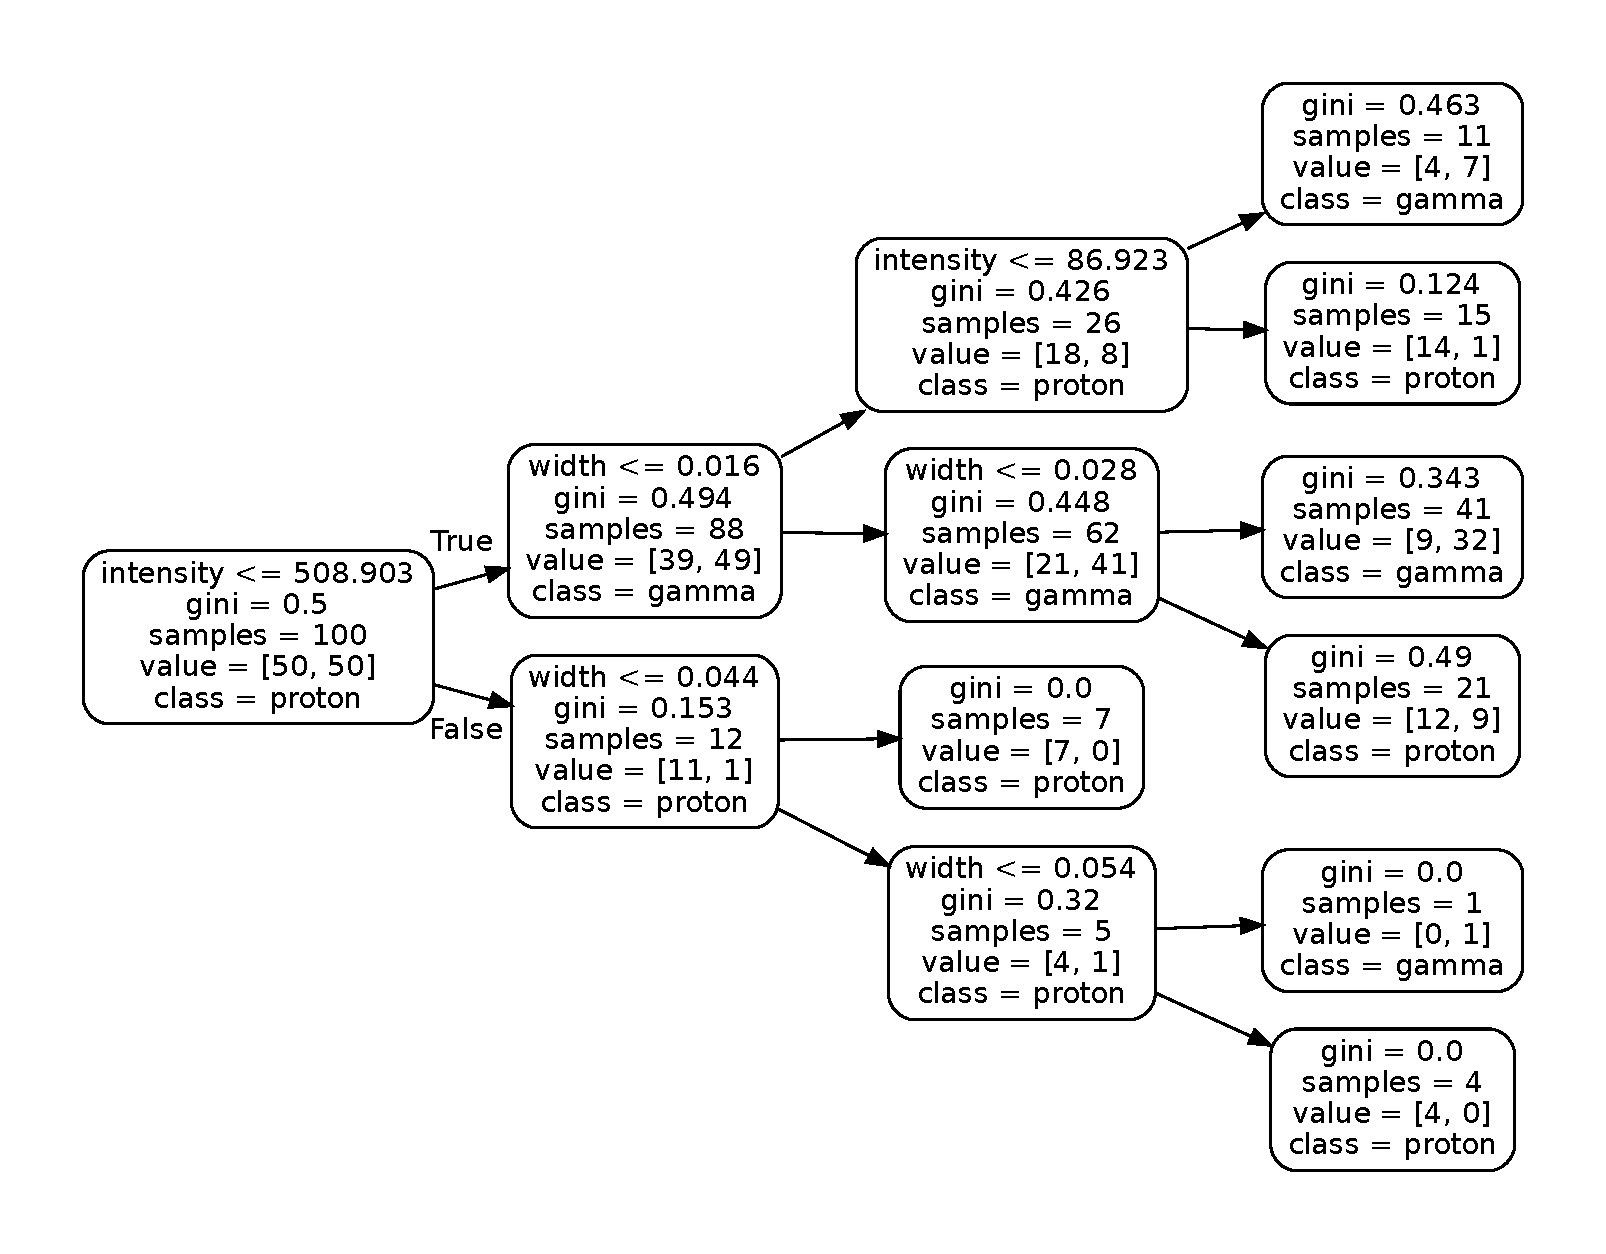
\includegraphics[width=.8\textwidth]{Plots/decision_tree.pdf}
    \caption{??}
    \label{fig:??}
\end{figure}

\begin{figure}
    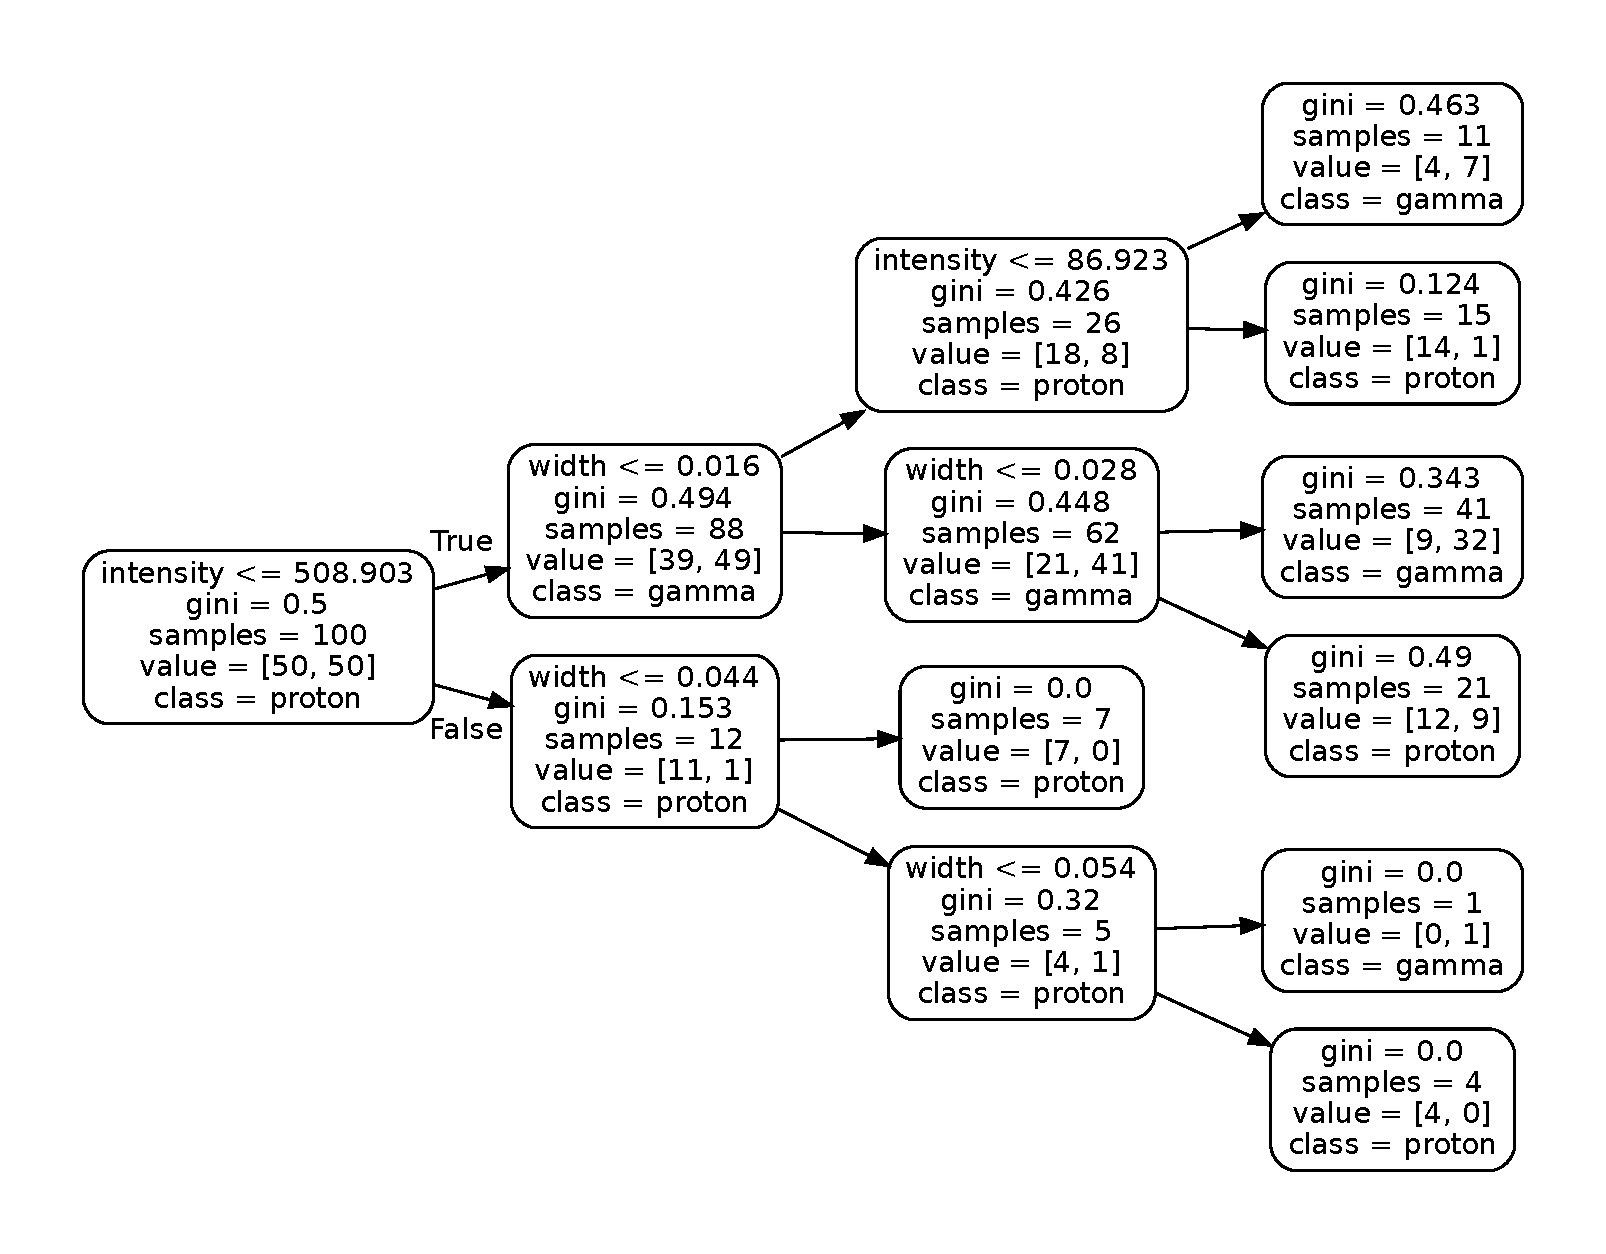
\includegraphics[width=.8\textwidth]{Plots/decision_tree.pdf}
    \caption{??}
    \label{fig:??}
\end{figure}

\begin{figure}
    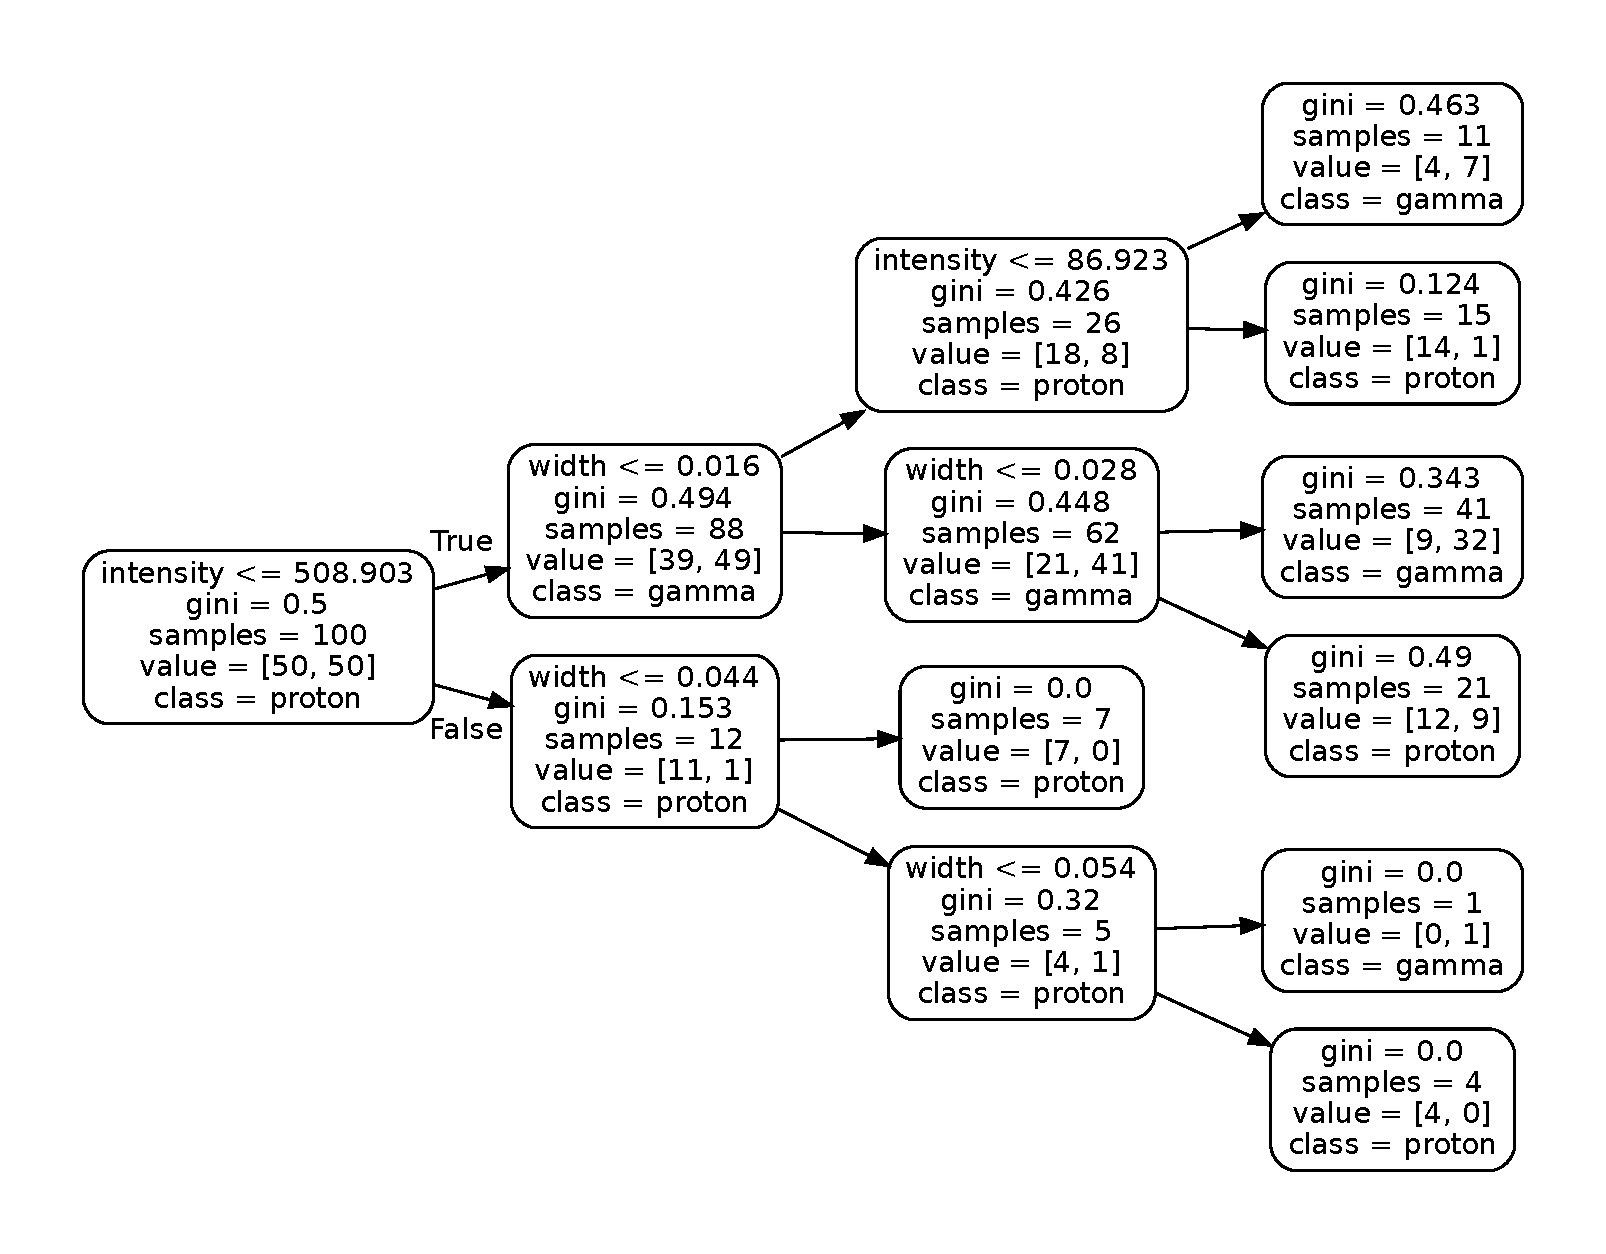
\includegraphics[width=.8\textwidth]{Plots/decision_tree.pdf}
    \caption{??}
    \label{fig:??}
\end{figure}

\begin{figure}
    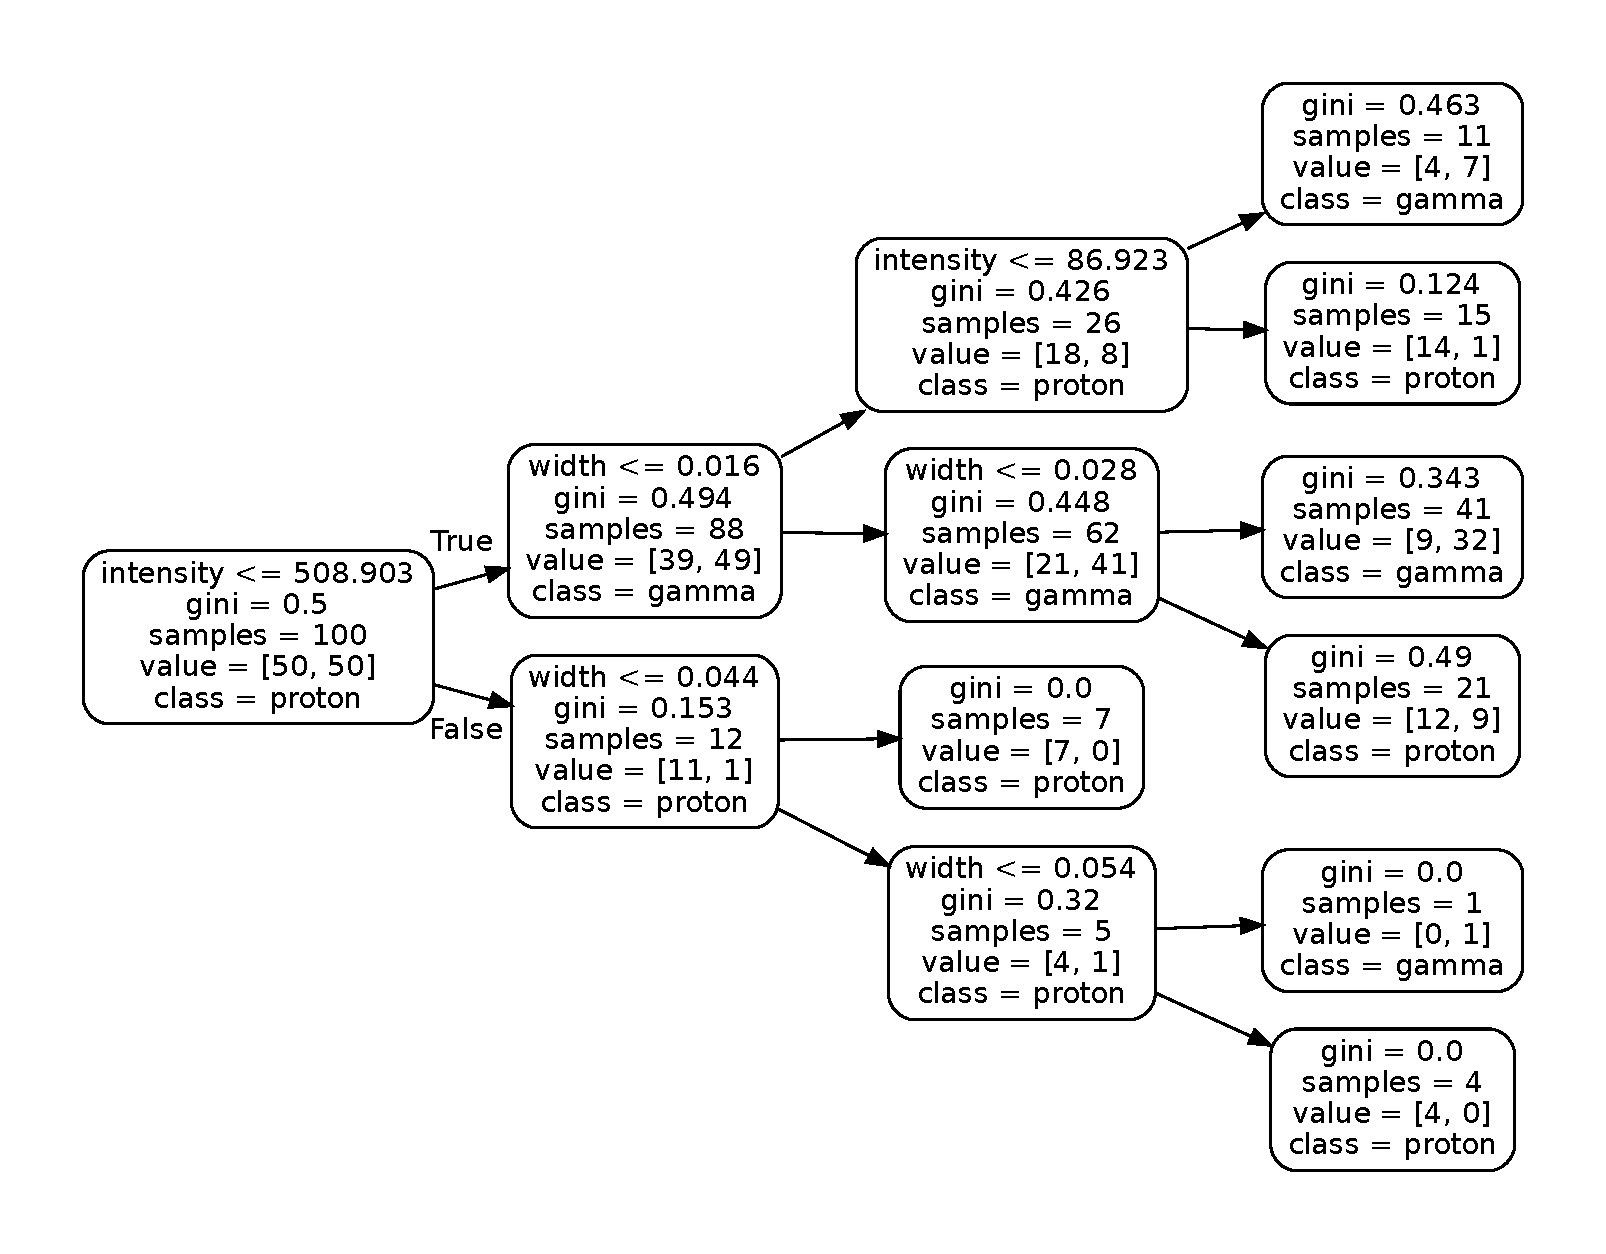
\includegraphics[width=.8\textwidth]{Plots/decision_tree.pdf}
    \caption{??}
    \label{fig:??}
\end{figure}



\subsection{Analysis for the stereoscopic array}
\begin{figure}
    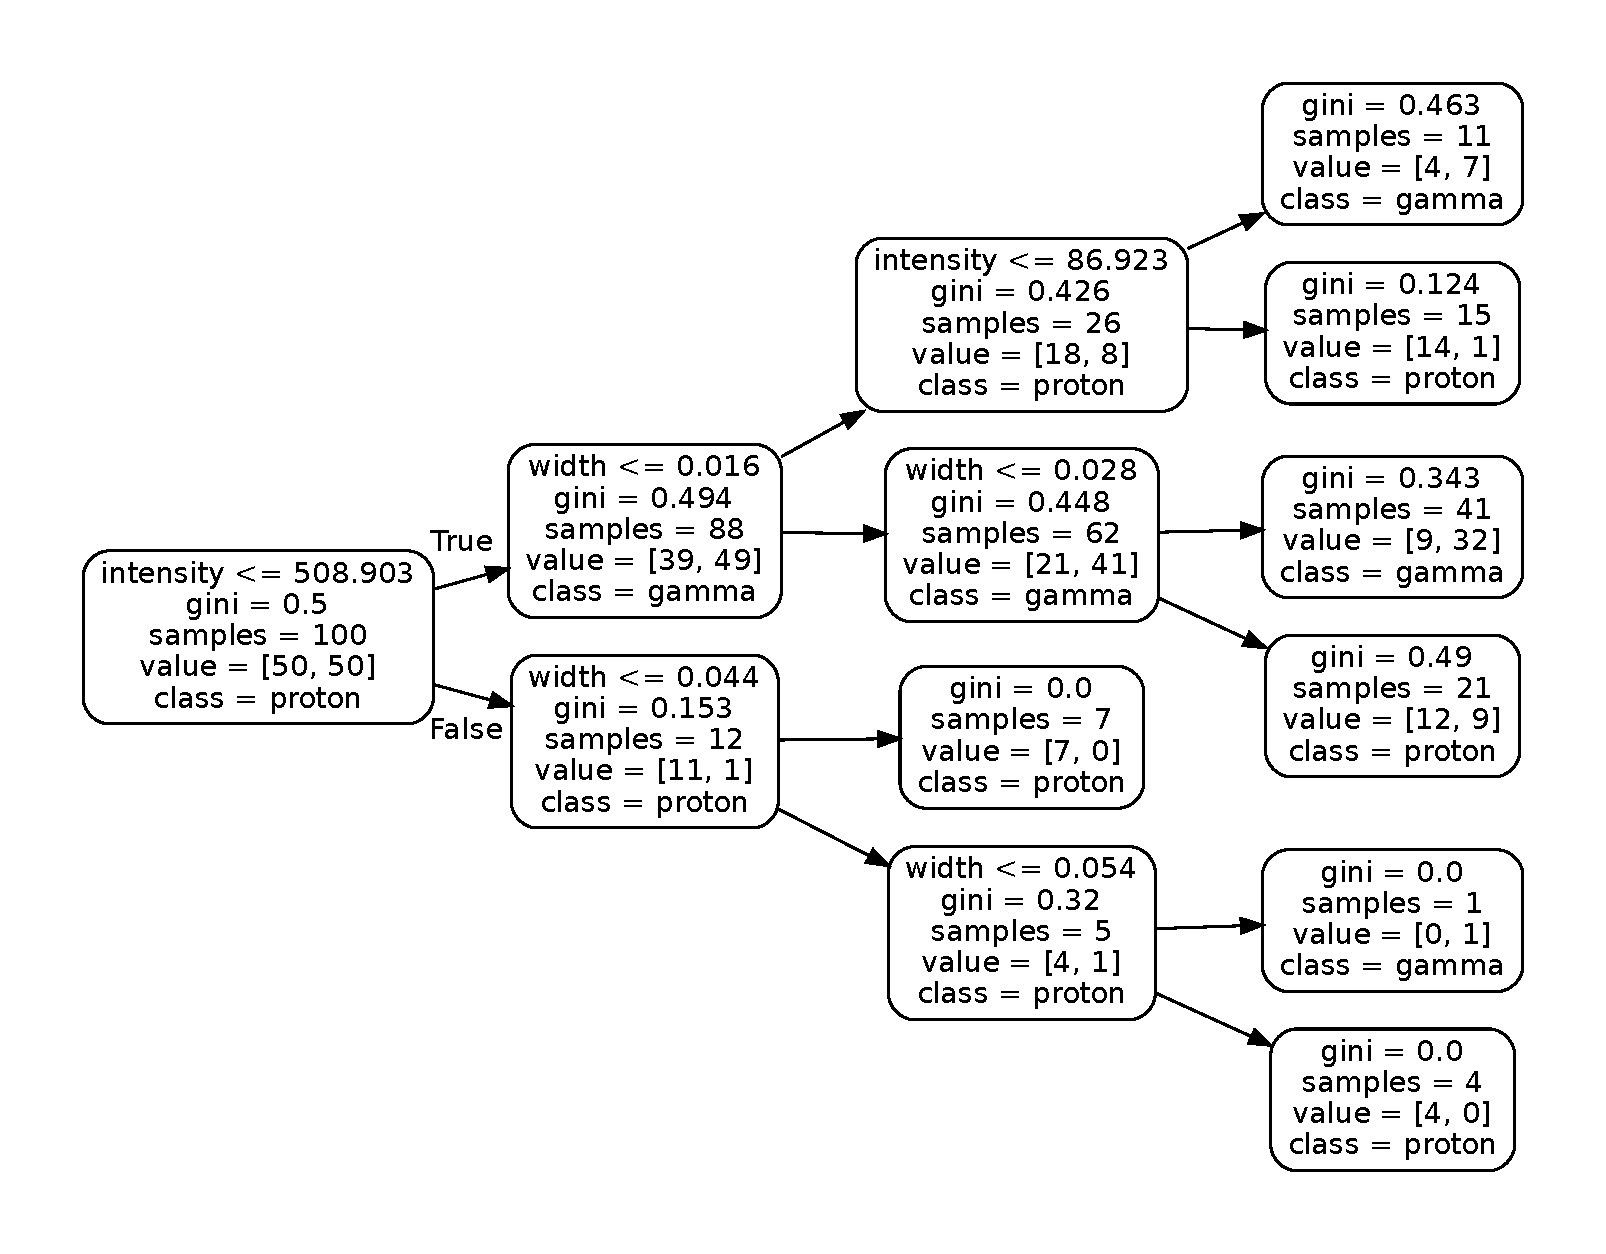
\includegraphics[width=.8\textwidth]{Plots/decision_tree.pdf}
    \caption{??}
    \label{fig:??}
\end{figure}

\begin{figure}
    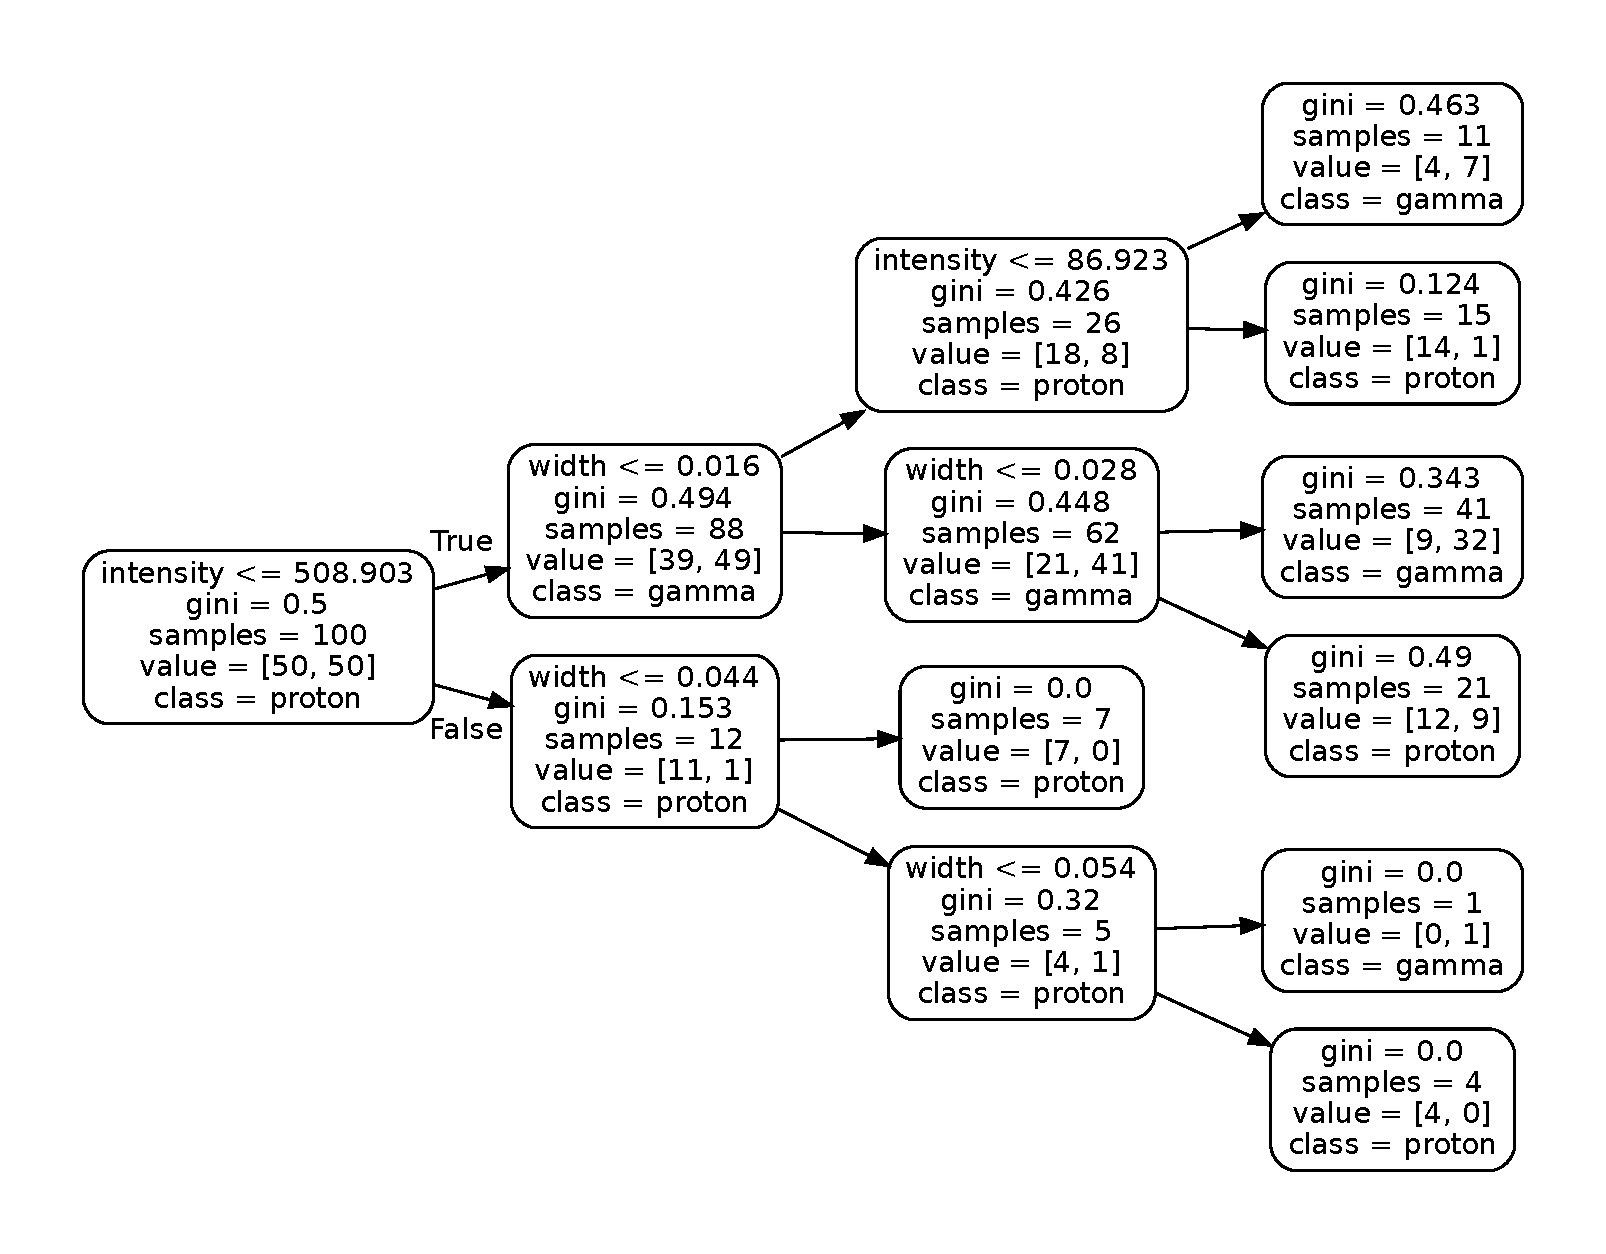
\includegraphics[width=.8\textwidth]{Plots/decision_tree.pdf}
    \caption{??}
    \label{fig:??}
\end{figure}

\begin{figure}
    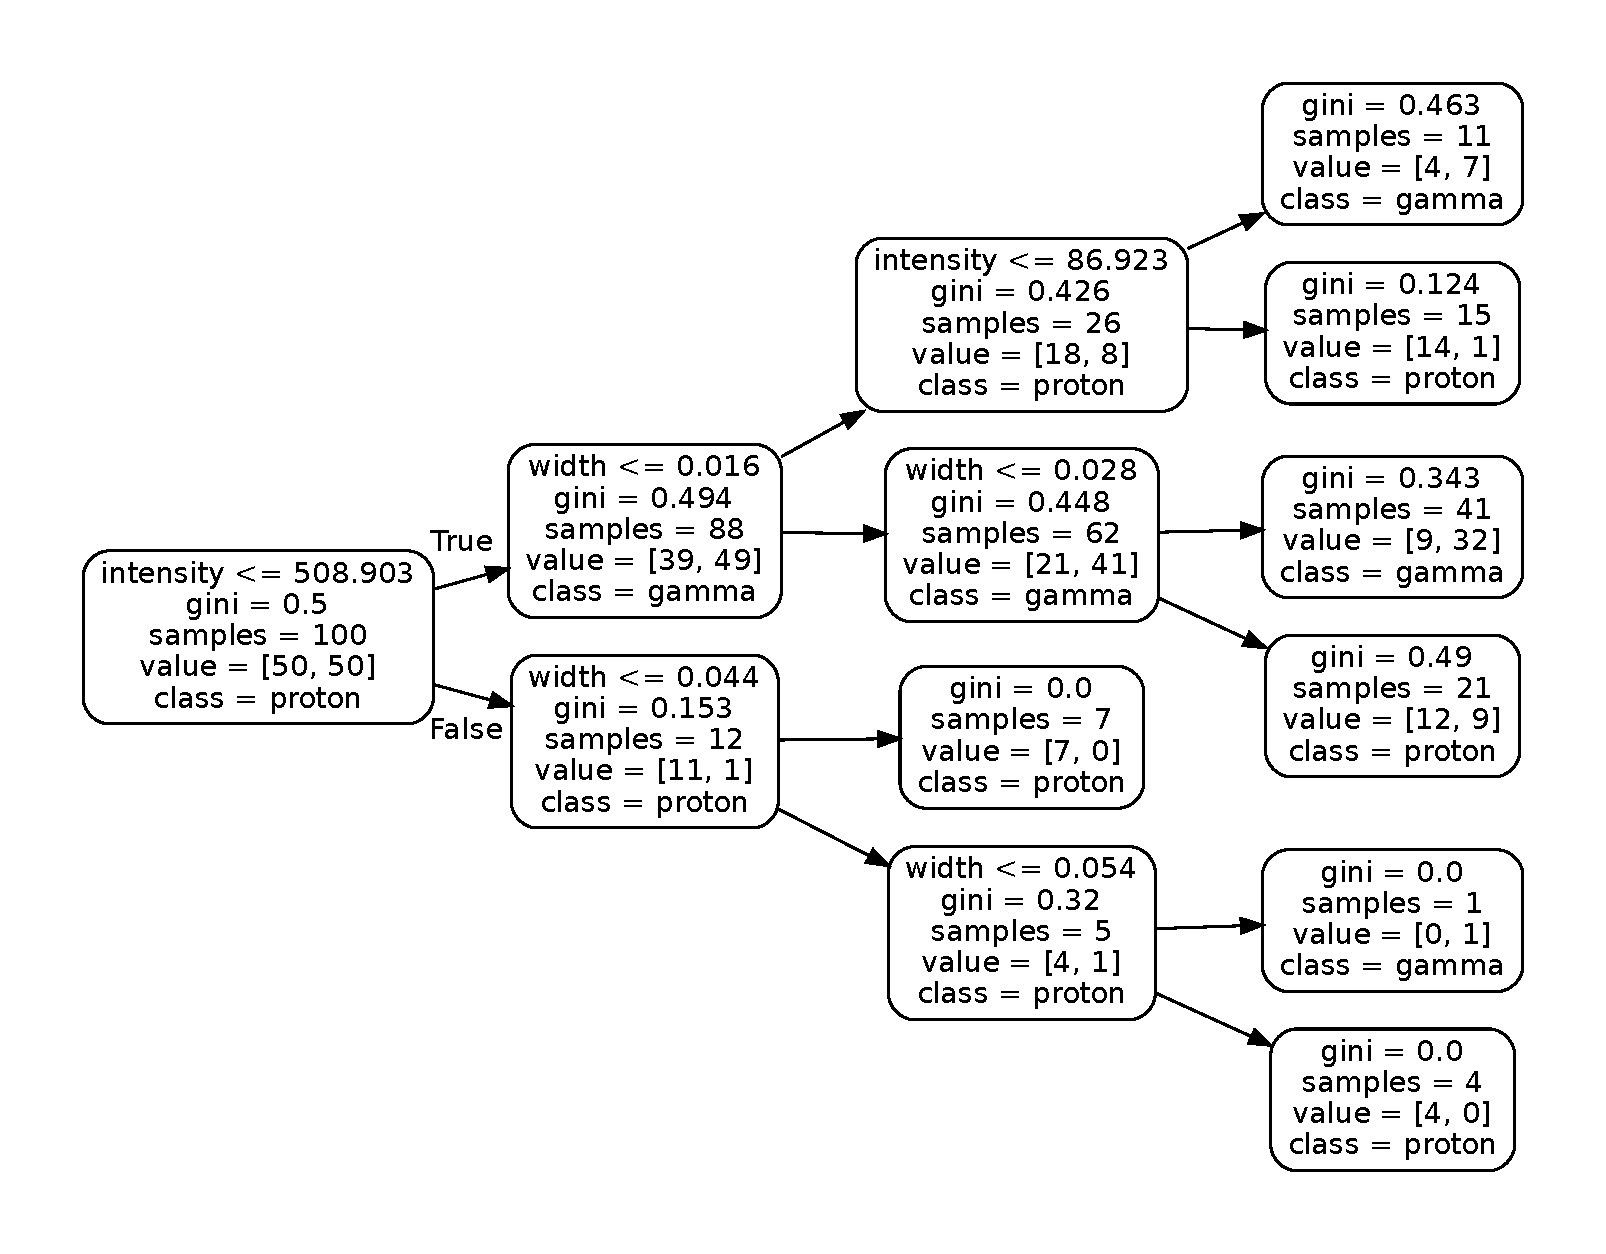
\includegraphics[width=.8\textwidth]{Plots/decision_tree.pdf}
    \caption{??}
    \label{fig:??}
\end{figure}

\begin{figure}
    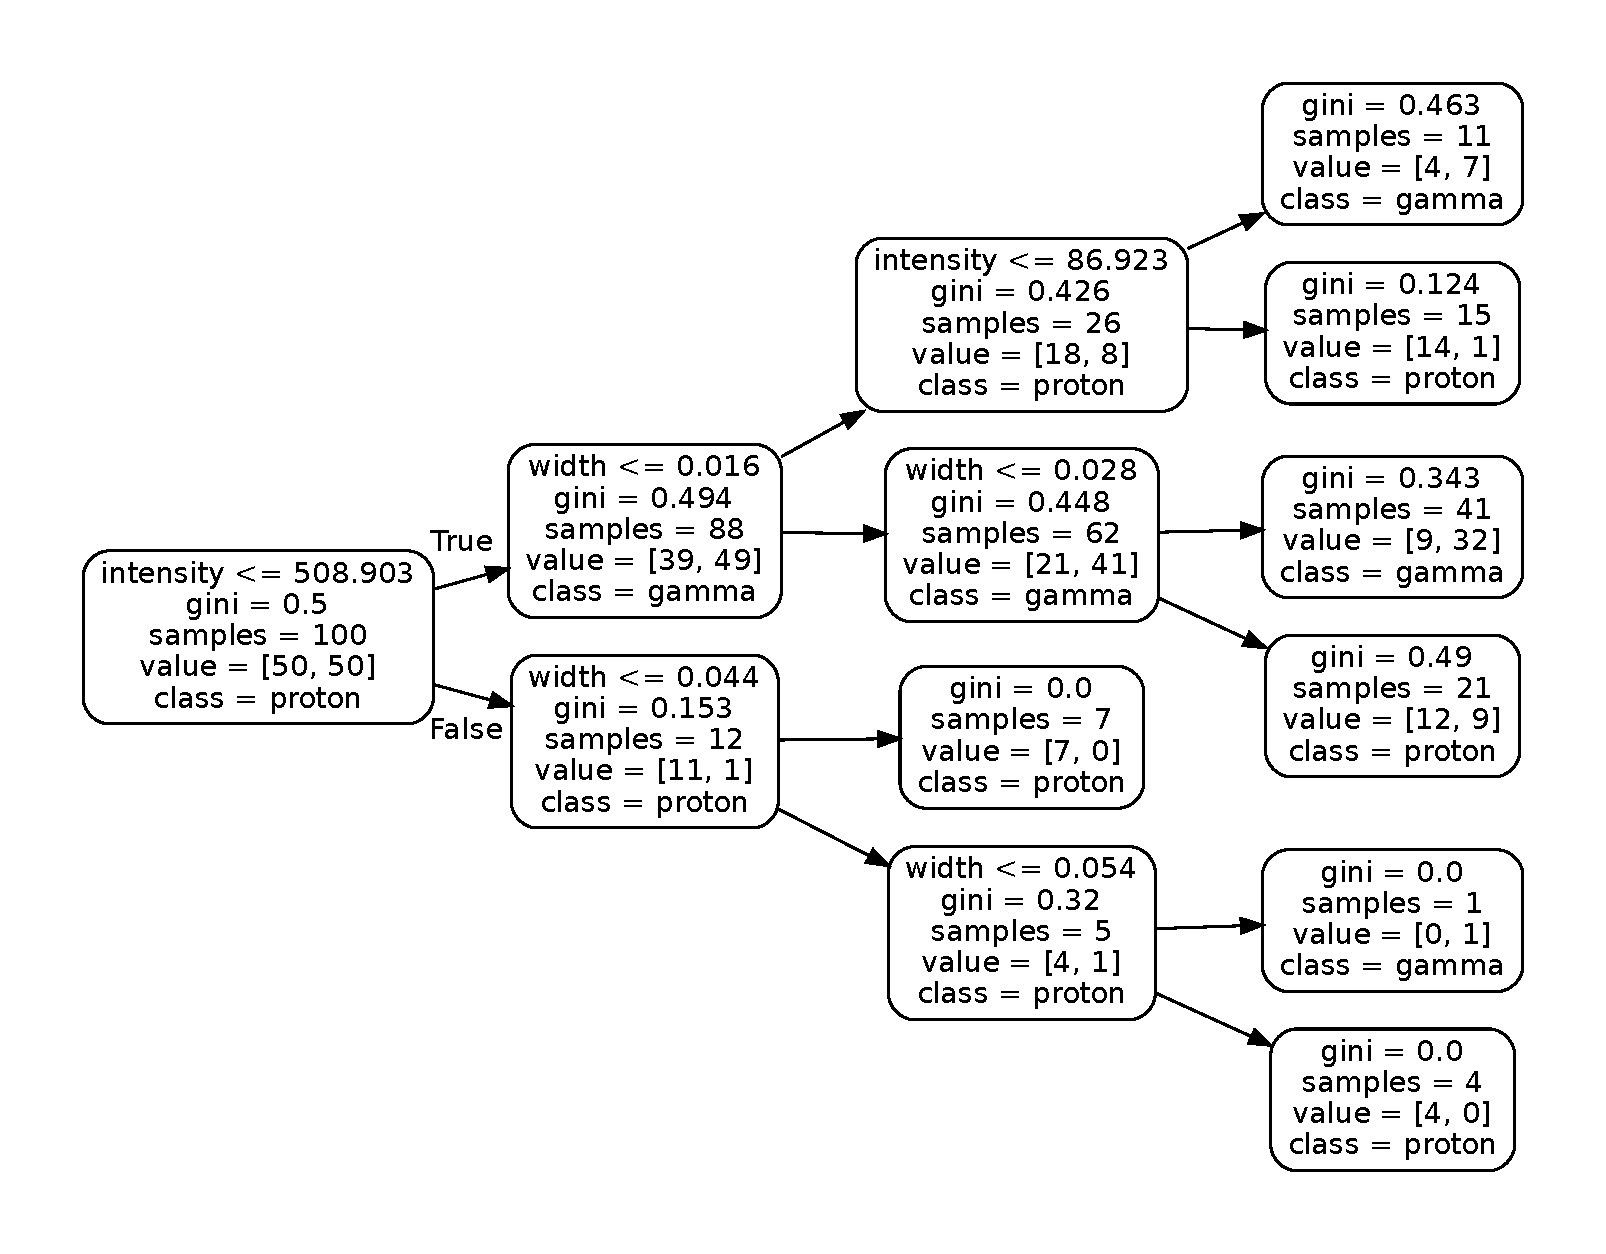
\includegraphics[width=.8\textwidth]{Plots/decision_tree.pdf}
    \caption{??}
    \label{fig:??}
\end{figure}


\subsubsection{hadroness cut}

\begin{figure}
    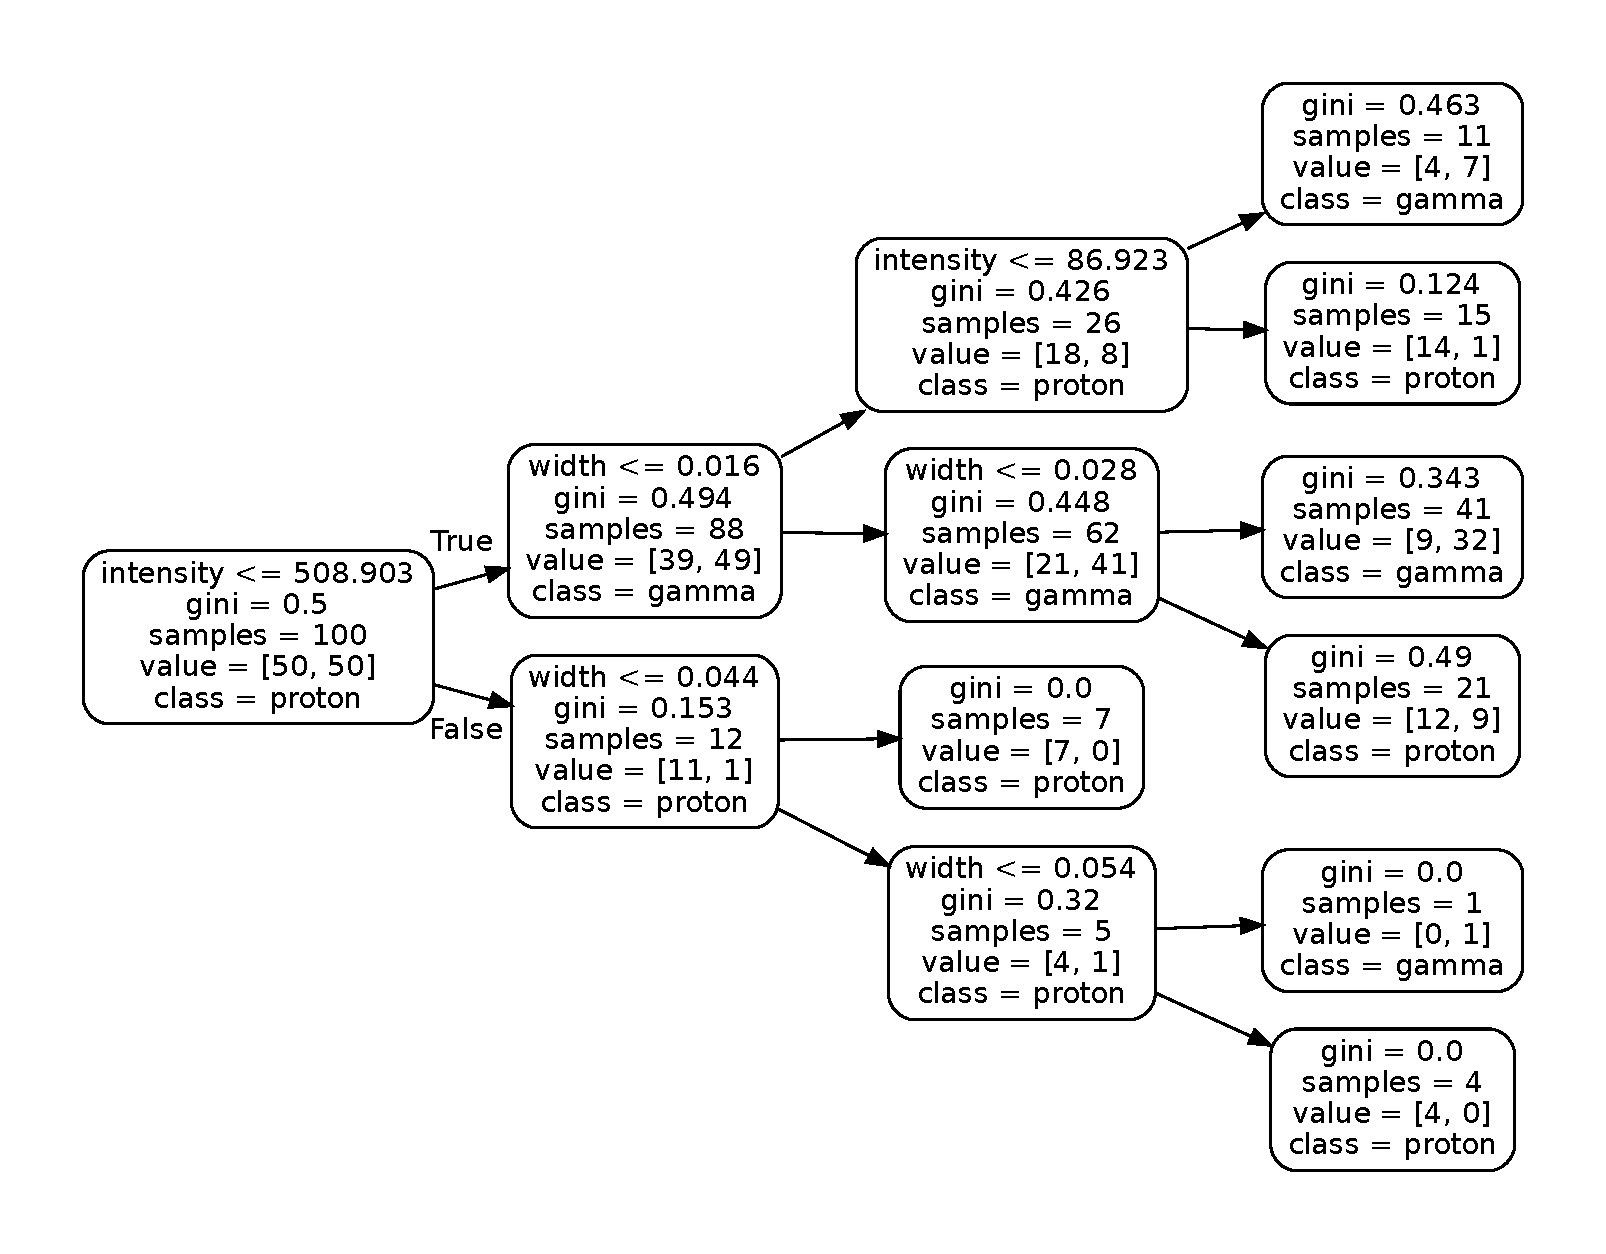
\includegraphics[width=.8\textwidth]{Plots/decision_tree.pdf}
    \caption{??}
    \label{fig:??}
\end{figure}

\begin{figure}
    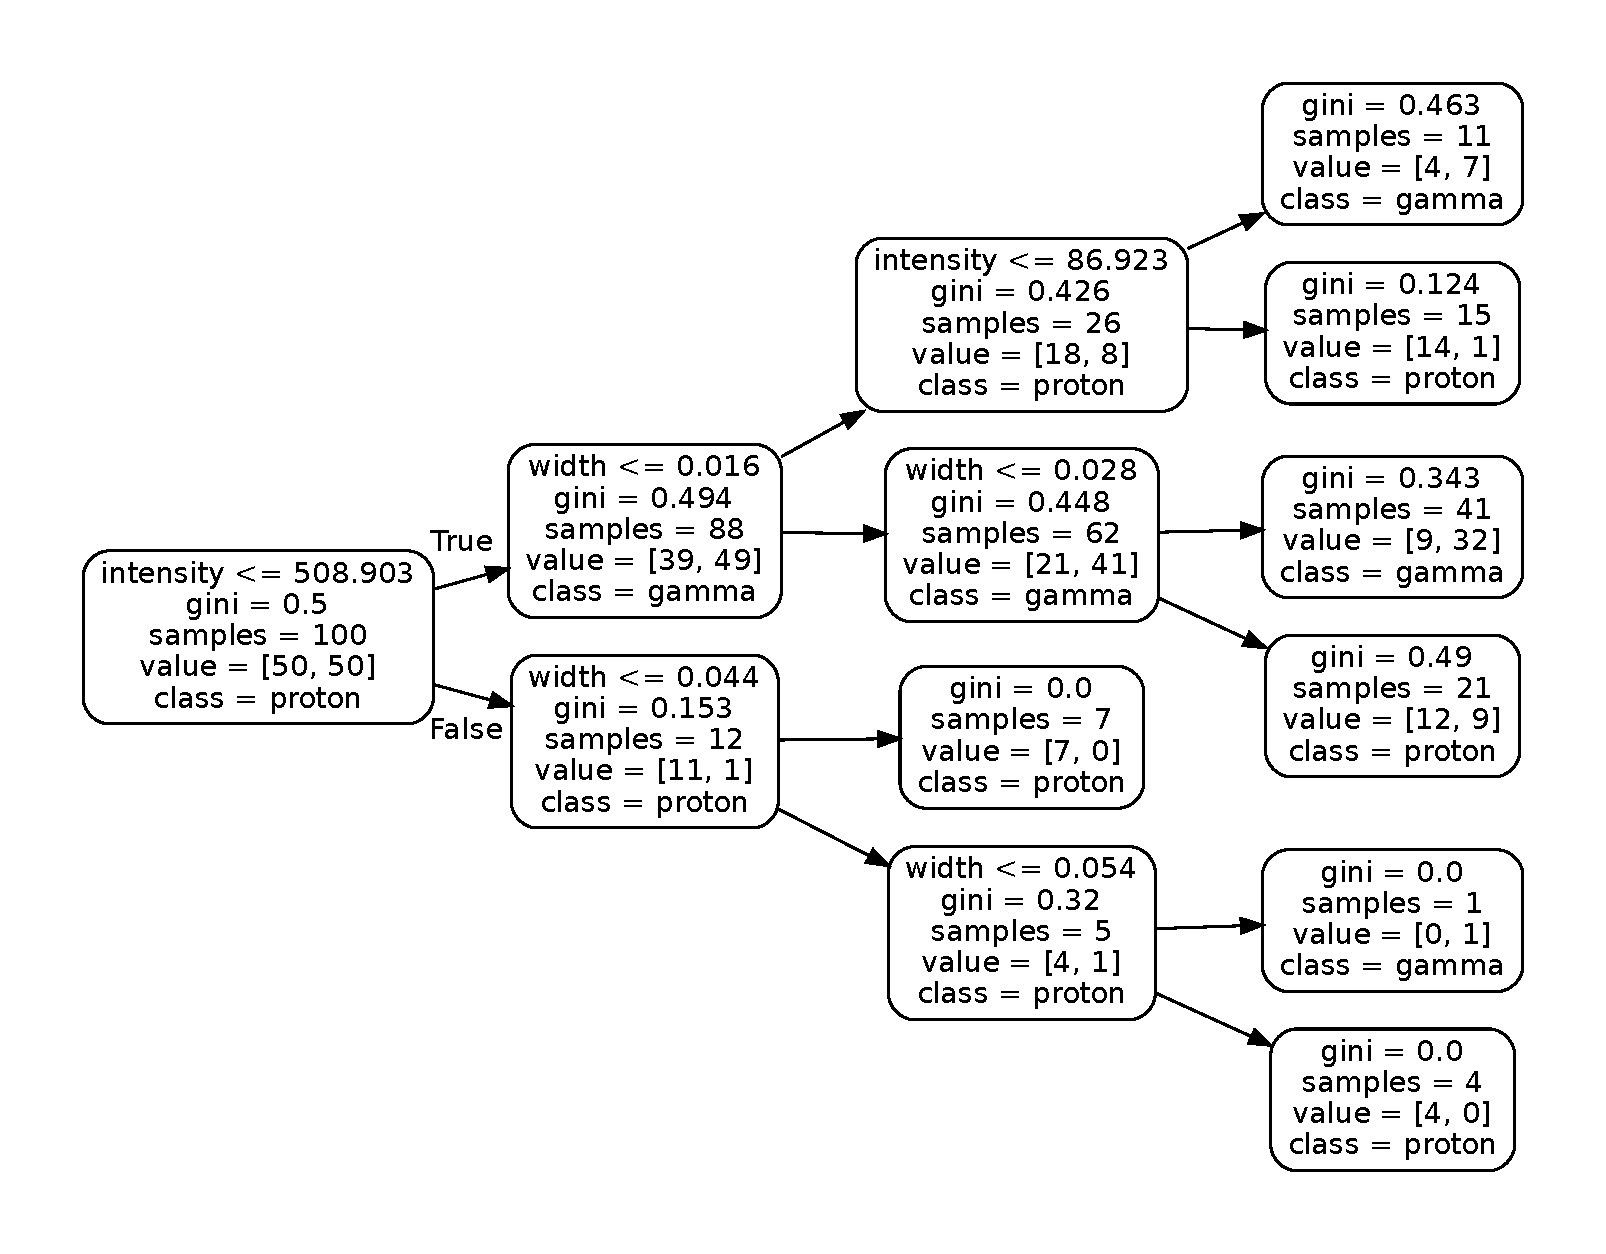
\includegraphics[width=.8\textwidth]{Plots/decision_tree.pdf}
    \caption{??}
    \label{fig:??}
\end{figure}

-> bringt nichts?